\documentclass[a4paper,man,natbib]{apa6}

\usepackage[english]{babel}
\usepackage[utf8x]{inputenc}
\usepackage{amsmath}
\usepackage{graphicx}
\usepackage[colorinlistoftodos]{todonotes}

\usepackage{multirow}
\usepackage{verbatim}
\usepackage{placeins}
\usepackage{float}
\usepackage{babel}
\restylefloat{figure}
\restylefloat{table}

\usepackage{tikz}
\usetikzlibrary{shapes,arrows}

% Modify Abstract title name from "Abstract" to "EXECUTIVE SUMMARY"
\addto{\captionsenglish}{\renewcommand{\abstractname}{EXECUTIVE SUMMARY}}

\title{\textbf{TROUBLESHOOTING AND DIAGNOSTIC ANALYSIS OF EARTH-MOVER SCRAPER --- CAT 637G}}
\shorttitle{CAT 637G --- Troubleshooting analysis }
\author{Prepared for

Lisa Slywka, Instructor

English and Communications

School of Applied Sciences and Technology
}
\affiliation{Prepared by

Tai Tran, 200222333

Industrial Heavy Equipment Technician Program

School of Applied Trades

October 31, 2016
}

%\abstract{}
    
\begin{document}

\centering The Northern Alberta Institute of Technology\\ Edmonton, Alberta

\maketitle

\tableofcontents
\newpage

\listoffigures
\newpage

\listoftables
\newpage



\section{INTRODUCTION}

% problem
``With today's highly sophisticated machinery and with the advent of mass production, industry can no longer afford a failure, as the cost of downtime is prohibitive.'' \citep[p. 190]{DodPracHyd}. To avoid these unexpected failures, techncians should recognize common symtoms and fix them before equipment breaks down.

\subsection{Purpose}

The goal of this report is to provide essential hydraulic and powertrain troubleshooting skills on Caterpillar scraper 637G. This research is significant due to the popularity of utilizing hydraulics in heavy equipment. As the vast majority of equipment heavily depends on hydraulics to do the job, including powertrain, technicians or students with troubleshooting skill in this field can consolidate their positions or increase the chances of getting a good job. In order to provide an in-depth analysis of the hydraulics and powertrain system, this report will not examine entire the 637G's hydraulic systems, which is not timely feasible.

\subsection{Background}

Just like a human body, if the owners and technicians neglect minor problems of equipment, things will get worse. Companies can have a comprehensive preventative maintenance strategy for their fleet; nevertheless, equipment still can fail at any time between service intervals because equipment health heavily relies on working environments. Hydraulic systems are very susceptible to contamination since components, such as cylinder seals are exposed to dusty environments. On the other hand, the powertrain might less prone to contamination as its components are less exposed. Therefore, their service life may be longer than other hydraulic systems, but their failures can cause longer downtime

%Understanding how to solve hydraulic and powertrain problems benefits both equipment owners and technicians. . 

\subsection{Scope}

Just like other heavy equipment, the 637G scraper uses hydraulics in many places: the bowl, apron, ejector, cushion-hitch, auger, steering, and powertrain. Because of the large amount of  hydraulic implementation used in the 637G, this paper will merely concentrate on the cushion-hitch, auger, and torque converter. Typically, the report will cover the purposes, locations, and basic diagnostic and troubleshooting knowledge for cushion-hitch, auger, and torque converter. Besides, the paper also incorporates safety procedures along with technical troubleshooting measures.

\section{EQUIPMENT DESCRIPTION}
\label{sec:examples}

\subsection{History Background}
 
``Invention of the scraper, as we know it today, is credited to Robert Gilmour LeTourneau, who had established his own earthmoving business in 1922.'' \citep[p. 59]{KthGnterth} Robert and his brother-in-law Ray Peterson built the first earthmoving scraper in June, 1922 in Stockton, California. After the first scraper was built by Letourneau in 1922, the author created a second version of earthmoving scraper, nicknamed the Gondola. Later, the third edition Mountain Mover was created in 1923. The self-propelled scraper was the fourth built. Letourneau continuously dedicated his life to improve his creations \citep{RLMBldng}.

\begin{figure}[!ht]
\centering
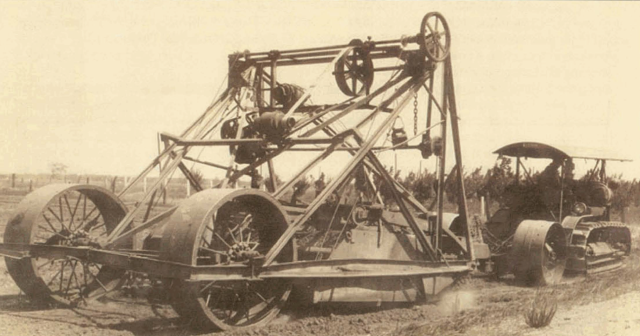
\includegraphics[width=\textwidth]{mountain_mover_1922.png}
\centering\caption{\label{fig:mmv}Mountain Mover with a telescoping bowl was invented in June, 1922. \citep{RLMBldng}}
\end{figure}

\subsection{Components}

The CAT 637G is a typical earthmoving scraper, designed for quick loading, hauling, dumping, and spreading of loose material. The below picture is a illustration of 637G.
\begin{figure}[!ht]
\centering
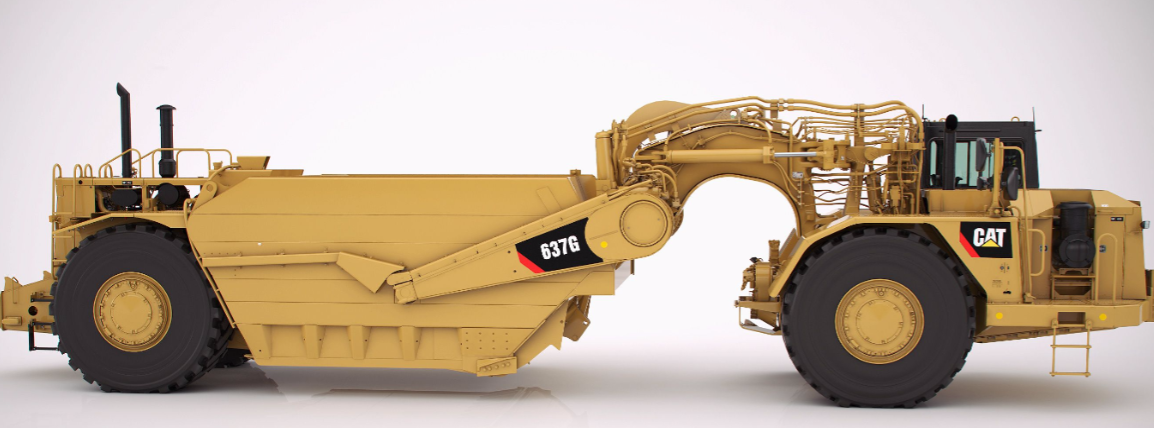
\includegraphics[width=\textwidth]{637G_scraper.png}
\centering\caption{\label{fig:crpr}A modern tractor earthmoving scraper Caterpillar 637G. \citep{THMPIndst}}
\end{figure}

The CAT 637G has a excellent self-loading capability in a wide range of material. It is designed to load material with auger mechanism which allows material distributed throughout the bowl. As shown in below figure, an earthmoving scraper has two parts: tractor and scraper.  
\begin{figure}[!ht]
\centering
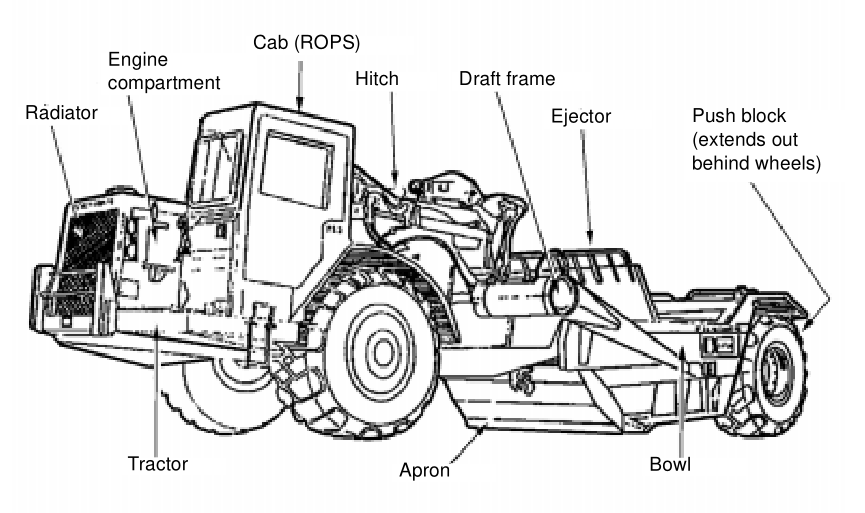
\includegraphics[width=\textwidth]{scraper_components.png}
\centering\caption{\label{fig:scprcmp}An illustration of scraper's components. \citep{DTMTrmy}}
\end{figure}

As shown above picture, a typical scraper has follwing components:
\begin{itemize}
\item A bowl is responsible for loading and carrying material with the help of cutting edge and auger mechanism. 
\item An auger in front of the bowl lifts material off of the cutting edge. It also helps to distribute material evenly throughout the bowl 
\item An apron mounted in font of the auger retains material upon hauling.
\item An ejector internally mounted in the end of the bowl helps to discharge material during spreading. 
\end{itemize}

\section{DIAGNOSTIC AND TROUBLESHOOTING ANALYSIS}

\subsection{Hydraulic Systems}

The 637G uses hydraulics in various places: steering, cushion-hitch, bowl, apron, ejector, auger, and bail. As mentioned in the previous section, only cushion-hitch and auger hydraulic systems will be examined.

\subsubsection{Cushion-hitch Hydraulic System and Service}

``The function of a cushion hitch system,\ldots, is to act as a connection device when it is mounted between the scraper.''\citep{GOASspns}. Below pictures taken from HeavyEquipment.org shows the left and right side of scraper gooseneck, cushion-hitch pump, and its control system. 

\begin{figure}[!ht]
\centering
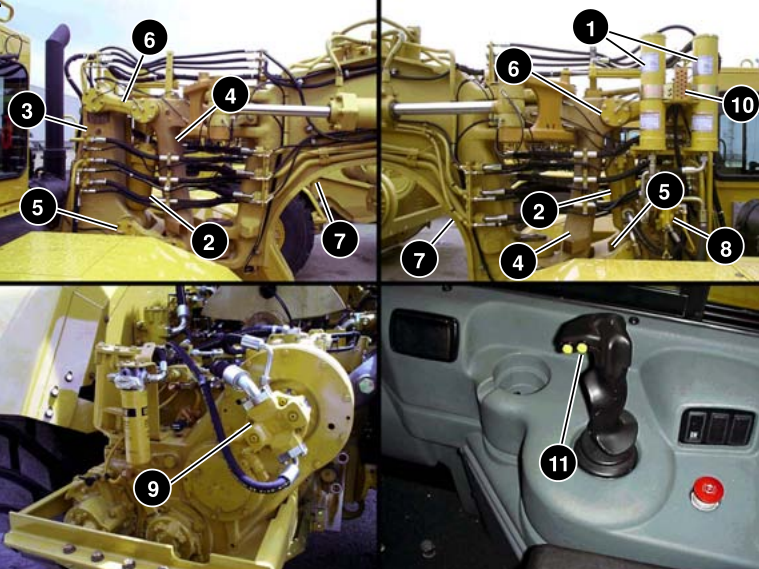
\includegraphics[width=\textwidth]{cushion-hitch-comp-location.png}
\centering\caption{\label{fig:cshh}Cushion-hitch hydraulic components. \citep{GOASspns}}
\end{figure}
\FloatBarrier{}

Cushion-hitch components includes following: (1) Accumulators, (2) Load cylinders, (3) Tractor bracket assembly, (4) Scraper hitch assembly, (5) Lower link, (6) Upper link, (7) Gooseneck, (8) Leveling valve, (9) Cushion-hitch pump, (10) Lubrication points, (11) Cushion-hitch button.


Two nitrogen accumulators help to dampen vertical movement by compressing nitrogen gas, and constantly providing oil back and forth to the load cylinder to stablize the equipment. The load cylinder lifts the hitch assembly off the tractor bracket in cushion ride mode. In lockdown mode, load cylinder is bottomed, providing a rigid connection between the scraper and tractor. As shown in below schematic taken from SIS portal, the 637G cushion-hitch features a load-sensing pump working with two accumulators.

\begin{figure}[!ht]
\centering
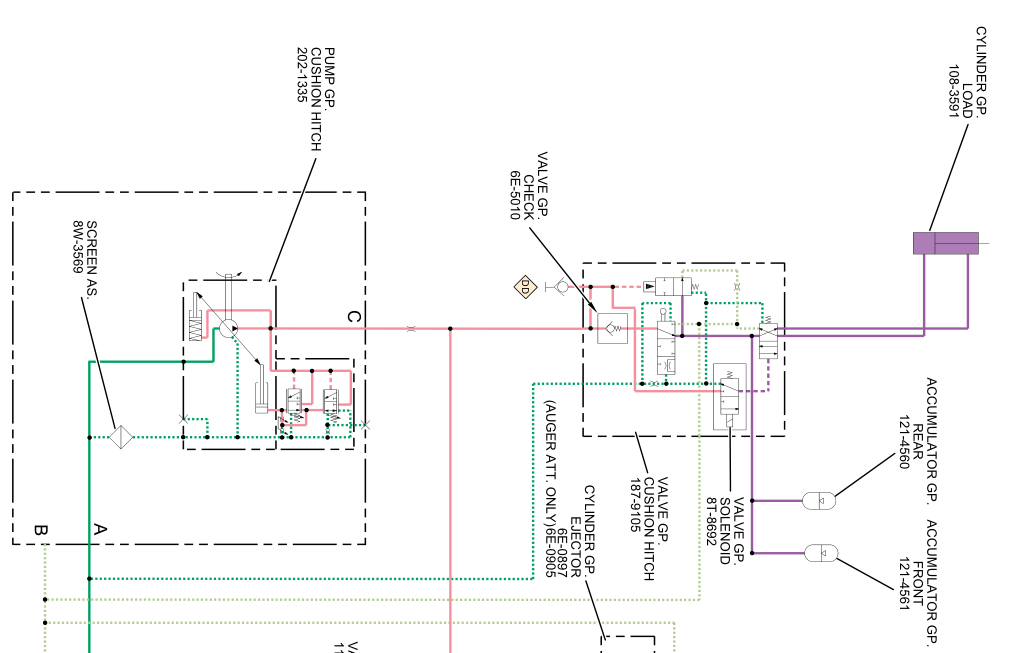
\includegraphics[scale=0.5, angle=90]{cushion-hitch.jpg}
\centering\caption{\label{fig:cshh}Cushion-hitch hydraulic system. \citep{SISCat}}
\end{figure}
\FloatBarrier{}

According to Caterpillar, as a rule of thumb, the first step of servicing any hydraulic systems, such as cushion-hitch, auger is to perform a visual inspection, which will help to identify any leakage, component damage, loose or missing components. After that, operation tests can be done to find leakage in the system, a failed valve or a failed pump. The hydraulic oil should be warmed up to 115 to 125F before performing do any test \citep{SISCat}. In order to reach normal operating temperature, operators have to run the engine at high idle for at least 5 minutes\citep{SISCat}. Below table shows common hydraulic faults and possible causes.

\begin{table}[!htbp]
\centering
\begin{tabular} {| l | l |}
\hline
Faults & Posible causes\\
\hline
\multirow{4}{10em}{Temperature of the hydraulic oil is excessively high} & --- The viscosity of the hydraulic oil is incorrect\\
& --- The cushion-hitch piston pump is excessively worn\\
& --- A restriction exists in a hydraulic oil passage\\
& --- An air restriction exists at the hydraulic oil cooler\\
\hline
\multirow{3}{10em}{There is a large amount of air in the oil} & --- There is a leak in the oil line between the tank and hydraulic pump.\\
& --- The return baffle in the tank is loose or broken.\\
& --- There is leakage around the cylinder seals.\\
\hline
\multirow{3}{10em}{The hydraulic and steering pump has no pressure} & --- Low level is low\\
& --- The hydraulic pump or pump drive shaft has malfunctioned.\\
& --- A relief valve has malfunctioned.\\
\hline
\multirow{3}{10em}{The cushion-hitch pump makes noise} & --- The viscosity of the oil is wrong.\\
& --- Loose connection of the oil line on the inlet side of the pump.\\
& --- The pump has too much wear.\\ 
\hline
\end{tabular}
\caption{\label{tab:chtblch}Common cushion-hitch problems and possible causes}
\end{table}
\FloatBarrier{}

\subsubsection{Auger Hydraulic System}

Following pictures taken from the HeavyEquipments.com manual shows the optional 637G's attachment: an auger.

\begin{figure}[!ht]
\centering
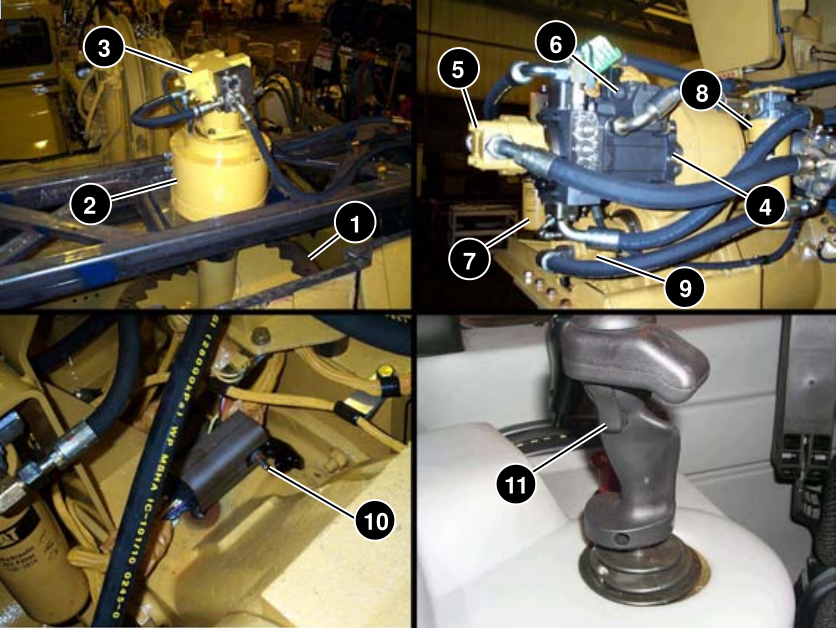
\includegraphics[width=\textwidth]{auger_comps.png}
\centering\caption{\label{fig:grcom}Hydraulic motors and control modules of auger is in the Caterpillar 637G \citep{hvyqpmtrg}}
\end{figure}
\FloatBarrier{}

\subsection{Powertrain}

\subsubsection{Torque Converter}

\section{CONCLUSION}



\bibliography{main}

\end{document}


